\chapter{Wektory i macierze}\label{rozdz:wektory}

\section{Dlaczego algebra liniowa?}

Prawie każda warstwa modelu Gen~6 to mnożenie przez macierz. Macierz zamienia jeden wektor cech na inny,
a iloczyn skalarny mierzy, jak bardzo dwa wektory są do siebie podobne; uwaga (rozdział~\ref{rozdz:uwaga})
to nic więcej niż iloczyny skalarne wstawione do softmaksa. Wystarczy nam kilka pojęć, ale musimy je rozumieć
geometrycznie.

Po tym rozdziale umiesz: (i)~policzyć iloczyn skalarny, normę i kąt, (ii)~uzasadnić nierówność Cauchy'ego--Schwarza,
(iii)~pomnożyć macierz przez wektor i dwie macierze przez siebie, (iv)~policzyć liczbę parametrów warstwy liniowej.

\section{Wektor i iloczyn skalarny}

\haslo{iloczyn skalarny}
\begin{definicja}[Iloczyn skalarny i norma]\label{def:iloczyn-skalarny}
Dla wektorów $\vect u,\vect v\in\R^n$ ich \emph{iloczynem skalarnym} jest liczba
\begin{equation}
  \ip{\vect u}{\vect v}=\sum_{i=1}^{n}u_iv_i=\vect u^{\top}\vect v ,
\end{equation}
a \emph{normą} (długością) wektora $\norm{\vect u}=\sqrt{\ip{\vect u}{\vect u}}$.
\end{definicja}

\begin{przyklad}\label{prz:iloczyn}
Dla $\vect u=(2,1,-1)$ i $\vect v=(1,3,2)$: $\ip{\vect u}{\vect v}=2\cdot1+1\cdot3+(-1)\cdot2=3$,
$\norm{\vect u}=\sqrt6\approx2{,}449$, $\norm{\vect v}=\sqrt{14}\approx3{,}742$. Iloczyn skalarny wektora z samym sobą
to kwadrat jego długości: $\ip{\vect u}{\vect u}=4+1+1=6$.
\end{przyklad}

\begin{intuicja}
Iloczyn skalarny pyta: „w ile wektor $\vect u$ jest skierowany tak jak $\vect v$?”. Wynik jest duży i dodatni,
gdy wskazują ten sam kierunek, zero, gdy są prostopadłe, ujemny, gdy przeciwne. W modelu wektor $\vect q$
(„czego szukam”) i wektor $\vect k$ („co mam”) są porównywane właśnie tak.
\end{intuicja}

\begin{twierdzenie}[Cauchy'ego--Schwarza]\label{tw:cs}
Dla dowolnych $\vect u,\vect v\in\R^n$ zachodzi $\abs{\ip{\vect u}{\vect v}}\le\norm{\vect u}\,\norm{\vect v}$, przy czym
równość jest równoważna temu, że wektory są równoległe (jeden jest wielokrotnością drugiego).
\end{twierdzenie}
\begin{pomyslDowodu}
Rozkładamy $\vect v$ na część równoległą do $\vect u$ i prostopadłą do niej. Część prostopadła ma nieujemną długość.
\end{pomyslDowodu}
\begin{proof}
Jeśli $\vect u=\vect0$, obie strony są zerem. Niech $\vect u\neq\vect0$ i niech $\vect p=\dfrac{\ip{\vect u}{\vect v}}{\norm{\vect u}^2}\vect u$
oraz $\vect r=\vect v-\vect p$. Sprawdzamy, że $\vect r\perp\vect u$:
\begin{align*}
\ip{\vect r}{\vect u} &= \ip{\vect v}{\vect u}-\frac{\ip{\vect u}{\vect v}}{\norm{\vect u}^2}\ip{\vect u}{\vect u} && \pow{(liniowość)}\\
 &= \ip{\vect u}{\vect v}-\ip{\vect u}{\vect v}=0. && \pow{($\ip{\vect u}{\vect u}=\norm{\vect u}^2$)}
\end{align*}
Skoro $\vect v=\vect p+\vect r$ z $\vect p\perp\vect r$, to $\norm{\vect v}^2=\norm{\vect p}^2+\norm{\vect r}^2\ge\norm{\vect p}^2$
(Pitagoras). A $\norm{\vect p}^2=\dfrac{\ip{\vect u}{\vect v}^2}{\norm{\vect u}^2}$, więc
\[
\norm{\vect v}^2\ge\frac{\ip{\vect u}{\vect v}^2}{\norm{\vect u}^2}
\quad\Longrightarrow\quad \ip{\vect u}{\vect v}^2\le\norm{\vect u}^2\norm{\vect v}^2 .
\]
Równość zachodzi dokładnie wtedy, gdy $\vect r=\vect0$, czyli $\vect v=\vect p$ jest wielokrotnością $\vect u$.
Pierwiastkowanie obu stron daje tezę.
\end{proof}

W zwykłym języku: iloczyn skalarny nigdy nie jest większy niż iloczyn długości, a największy jest dla wektorów
równoległych. Stąd wynika, że liczba $\cos\theta:=\ip{\vect u}{\vect v}/(\norm{\vect u}\norm{\vect v})$ leży w $[-1,1]$
i można ją nazwać cosinusem kąta $\theta$ między wektorami (rys.~\ref{rys:rzut}). Tę samą nierówność wykorzystamy
w rozdziale~\ref{rozdz:pochodne}, by pokazać, w którą stronę gradient rośnie najszybciej.

\begin{figure}[ht]
\centering
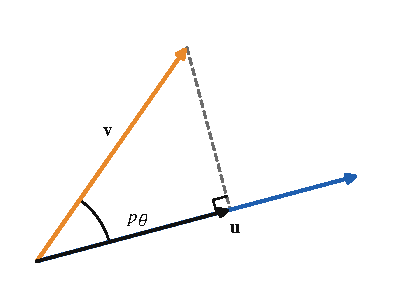
\includegraphics[width=\linewidth]{figures/rzut.pdf}
\sidecaption{Rozkład z dowodu tw.~\ref{tw:cs}. Wektor $\vect v$ (pomarańczowy) rzutujemy na kierunek $\vect u$ (niebieski):
rzut $p$ (czarny) jest równoległy do $\vect u$, a odcinek kreskowany $\vect r=\vect v-\vect p$ jest do niego prostopadły (kąt prosty).
Długość rzutu to $\norm{\vect v}\cos\theta$, więc $\ip{\vect u}{\vect v}=\norm{\vect u}\norm{\vect v}\cos\theta$. \label{rys:rzut}}
\end{figure}

\begin{naliczbach}
Dla wektorów z przykładu~\ref{prz:iloczyn}: $\cos\theta=3/\sqrt{6\cdot14}=3/9{,}165=0{,}327$, czyli $\theta\approx70{,}9^\circ$.
Rzut $\vect v$ na $\vect u$ to $\vect p=\frac{3}{6}\vect u=(1;\,0{,}5;\,-0{,}5)$, a reszta $\vect r=\vect v-\vect p=(0;\,2{,}5;\,2{,}5)$.
Sprawdzenie prostopadłości: $\ip{\vect r}{\vect u}=0\cdot2+2{,}5\cdot1+2{,}5\cdot(-1)=0$. \checkmark
\end{naliczbach}

\begin{pulapka}
Iloczyn skalarny rośnie wraz z długością wektorów, nie tylko z podobieństwem kierunków. Dwa długie, słabo
podobne wektory mogą mieć większy iloczyn niż dwa krótkie, równoległe. Dlatego w uwadze dzielimy iloczyn przez
$\sqrt{d_h}$ (rozdział~\ref{rozdz:uwaga}), a w sieci normalizujemy cechy (rozdział~\ref{rozdz:siec}).
\end{pulapka}

\section{Macierz jako przekształcenie}

\haslo{macierz}
\begin{definicja}[Iloczyn macierzy i wektora]\label{def:macierz-wektor}
Dla macierzy $W\in\R^{m\times n}$ i wektora $\vect x\in\R^n$ wektor $W\vect x\in\R^m$ ma współrzędne
\begin{equation}
  (W\vect x)_i=\sum_{j=1}^{n}W_{ij}x_j=\ip{\vect w_i}{\vect x},
\end{equation}
gdzie $\vect w_i$ to $i$-ty wiersz $W$. Każda współrzędna wyniku to iloczyn skalarny wiersza z wektorem.
\end{definicja}

\begin{przyklad}\label{prz:macierz-wektor}
Niech $W=\begin{pmatrix}1&2\\0&1\\-1&1\end{pmatrix}\in\R^{3\times2}$ i $\vect x=(2,1)$. Wtedy
$W\vect x=(1\cdot2+2\cdot1,\ 0\cdot2+1\cdot1,\ -1\cdot2+1\cdot1)=(4,1,-1)$: wektor z $\R^2$ trafił do $\R^3$.
Dodając wektor obciążenia (ang.\ \emph{bias}) $\vect b=(0{,}5;0;1)$ dostajemy \emph{warstwę liniową}
$W\vect x+\vect b=(4{,}5;\,1;\,0)$.
\end{przyklad}

\begin{intuicja}
Macierz $2\times2$ działa na całą płaszczyznę naraz: prosta zostaje prostą, początek układu zostaje na miejscu, a
siatka kwadratów zamienia się w siatkę równoległoboków. Kolumny $W$ to obrazy wektorów bazowych (rys.~\ref{rys:macierz-siatka}).
\end{intuicja}

\begin{figure*}[ht]
\centering
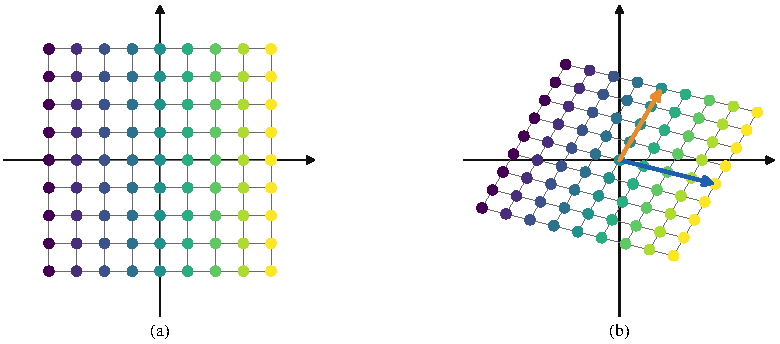
\includegraphics[width=\linewidth]{figures/macierz-siatka.pdf}
\caption{(a) Siatka punktów $9\times9$ w kwadracie $[-1,1]^2$, pokolorowana według współrzędnej $x$ (od fioletu do żółci).
(b) Obraz tej siatki po przekształceniu $\vect x\mapsto A\vect x$ z kolumnami $A\vect e_1$ (niebieska strzałka) i $A\vect e_2$
(pomarańczowa). Kolory pozwalają śledzić każdy punkt: proste zostają prostymi, a pole kwadratu rośnie $\abs{\det A}=1{,}2\cdot1{,}6+0{,}7\cdot0{,}4=2{,}2$ razy.}
\label{rys:macierz-siatka}
\end{figure*}

\begin{twierdzenie}[Mnożenie macierzy to składanie przekształceń]\label{tw:mnozenie}
Dla $A\in\R^{m\times n}$ i $B\in\R^{n\times p}$ macierz $AB\in\R^{m\times p}$ o elementach
$(AB)_{ik}=\sum_{j}A_{ij}B_{jk}$ spełnia $(AB)\vect x=A(B\vect x)$ dla każdego $\vect x\in\R^p$.
\end{twierdzenie}
\begin{pomyslDowodu}
Rozpisujemy obie strony na współrzędne i zamieniamy kolejność sumowania.
\end{pomyslDowodu}
\begin{proof}
\begin{align*}
\big(A(B\vect x)\big)_i &= \sum_{j=1}^{n}A_{ij}\,(B\vect x)_j && \pow{(def.~\ref{def:macierz-wektor})}\\
 &= \sum_{j=1}^{n}A_{ij}\sum_{k=1}^{p}B_{jk}x_k && \pow{(def.~\ref{def:macierz-wektor})}\\
 &= \sum_{k=1}^{p}\Big(\sum_{j=1}^{n}A_{ij}B_{jk}\Big)x_k && \pow{(zmiana kolejności sum)}\\
 &= \sum_{k=1}^{p}(AB)_{ik}\,x_k=\big((AB)\vect x\big)_i. && \pow{(def.\ $AB$)}
\end{align*}
Obie strony mają te same współrzędne, więc są równe. Wymiary zgadzają się, bo $B\vect x\in\R^n$, a $A$ przyjmuje wektory z $\R^n$.
\end{proof}

W zwykłym języku: dwie warstwy liniowe pod rząd to jedna warstwa liniowa o macierzy $AB$. Dlatego sieci wstawiają między
warstwy funkcje nieliniowe (rozdział~\ref{rozdz:siec}); bez nich głębokość nic by nie dała.

\begin{przyklad}[Kolejność ma znaczenie]\label{prz:nieprzemienne}
Dla $A=\begin{pmatrix}1&1\\0&1\end{pmatrix}$ i $B=\begin{pmatrix}2&0\\1&1\end{pmatrix}$ mamy
$AB=\begin{pmatrix}3&1\\1&1\end{pmatrix}$, ale $BA=\begin{pmatrix}2&2\\1&2\end{pmatrix}$. Mnożenie macierzy nie jest przemienne.
\end{przyklad}

\section{Ile parametrów ma warstwa?}

Warstwa liniowa $\vect x\mapsto W\vect x+\vect b$ z $n$ wejściami i $m$ wyjściami ma $mn+m$ parametrów
($W$ ma $mn$ liczb, $\vect b$ ma $m$). To najprostszy rachunek, który będziemy powtarzać w dodatku~\ref{dod:parametry}.

\begin{naliczbach}
Warstwa $64\to256$ (pierwsza w bloku feed-forward modelu Gen~6): $256\cdot64+256=16\,640$ parametrów. Warstwa
$256\to64$: $64\cdot256+64=16\,448$. Razem blok ma $33\,088$ parametrów.
\end{naliczbach}

\section*{Podsumowanie}
\begin{itemize}
\item $\ip{\vect u}{\vect v}=\sum u_iv_i=\norm{\vect u}\norm{\vect v}\cos\theta$ mierzy zgodność kierunków (tw.~\ref{tw:cs}).
\item Rzut $\vect v$ na $\vect u$ to $\frac{\ip{\vect u}{\vect v}}{\norm{\vect u}^2}\vect u$; reszta jest prostopadła do $\vect u$.
\item $W\vect x$: każda współrzędna to iloczyn skalarny wiersza z wektorem; $m\times n$ to $n\to m$.
\item $(AB)\vect x=A(B\vect x)$; mnożenie macierzy nie jest przemienne.
\item Warstwa liniowa $n\to m$ ma $mn+m$ parametrów.
\end{itemize}

\begin{sprawdz}
\begin{enumerate}
\item Dla $\vect u=(1,2,2)$ i $\vect v=(2,0,1)$ policz $\ip{\vect u}{\vect v}$, obie normy i $\cos\theta$. Czy wektory są prostopadłe?
\item Znajdź wektor $\vect w$ prostopadły do $\vect u=(1,2,2)$, taki że $\vect w=(a,1,0)$.
\item Policz $AB$ dla $A=\begin{pmatrix}2&0\\1&1\end{pmatrix}$, $B=\begin{pmatrix}1&3\\0&2\end{pmatrix}$ i sprawdź tw.~\ref{tw:mnozenie} dla $\vect x=(1,1)$.
\item Ile parametrów ma warstwa $159\to48$? A konwolucja $1\times1$ z $336$ kanałów do $48$ (zob.\ rozdz.~\ref{rozdz:siec})?
\end{enumerate}
\end{sprawdz}

\subsection*{Rozwiązania}
\begin{enumerate}
\item $\ip{\vect u}{\vect v}=2+0+2=4$, $\norm{\vect u}=3$, $\norm{\vect v}=\sqrt5$, $\cos\theta=4/(3\sqrt5)=0{,}596$. Nie są prostopadłe (iloczyn $\neq0$).
\item $\ip{\vect u}{\vect w}=a+2=0$, więc $a=-2$ i $\vect w=(-2,1,0)$.
\item $AB=\begin{pmatrix}2&6\\1&5\end{pmatrix}$. $AB\vect x=(8,6)$; $B\vect x=(4,2)$, $A(B\vect x)=(8,\,4+2)=(8,6)$. \checkmark
\item $159\cdot48+48=7680$. Konwolucja $1\times1$ to warstwa liniowa w każdym punkcie: $336\cdot48+48=16\,176$ parametrów.
\end{enumerate}
